
%! program = pdflatex

\documentclass[12pt]{article}
\usepackage{amsmath}
\usepackage{natbib}
\usepackage{graphicx}
\usepackage{amssymb}
\usepackage{epstopdf}
\usepackage{float} % to keep the figures in place
\usepackage{placeins}

\usepackage{caption}
\usepackage{subcaption}
\usepackage{color}
\usepackage{undertilde}
\usepackage{enumitem}
\newcommand{\cred}{ \color{red}}
\newcommand{\cgreen}{\color{green}}
\newcommand{\cblue}{\color{blue}}
\newcommand{\cmag}{\color{magenta}}
\newcommand{\bn}{\begin{enumerate}}
\newcommand{\en}{\end{enumerate}}
\newcommand{\bi}{\begin{itemize}}
\newcommand{\ei}{\end{itemize}}
\newcommand{\be}{\begin{eqnarray}}
\newcommand{\ee}{\end{eqnarray}}
\newcommand{\by}{\begin{eqnarray*}}
\newcommand{\ey}{\end{eqnarray*}}
\renewcommand{\labelenumi}{(\alph{enumi}) }
%
\usepackage[margin=2.2cm, includehead]{geometry}% see geometry.pdf on how to lay out the page. There's lots.
\geometry{letterpaper} % or letter or a5paper or ... etc
% \geometry{landscape} % rotated page geometry
%\bibpunct{(}{)}{;}{a}{,}{,}
%\setlength{\textwidth}{16cm}
%\setlength{\textheight}{21cm}
\def\nonumber{\global\@eqnswfalse}
\newcounter{parnum}
\newcommand{\N}{%
  \noindent\refstepcounter{parnum}%
   \makebox[\parindent][l]{\textbf{[\arabic{parnum}]}}\quad  }
% Use a generous paragraph indent so numbers can be fit inside the
% indentation space.
\setlength{\parindent}{1.5em}

% See the ``Article customise'' template for come common customisations

\date{}
%\date{} % delete this line to display the current date

%%% BEGIN DOCUMENT
\usepackage{Sweave}
\begin{document}
\Sconcordance{concordance:aua257HW1.tex:aua257HW1.Rnw:%
1 52 1 1 0 125 1}

%\large
%\maketitle
\newtheorem{thm}{Theorem}[section]
\newtheorem{cor}[thm]{Corollary}
\newtheorem{lem}[thm]{Lemma}
\newtheorem{prop}[thm]{Proposition}
\newtheorem{defn}[thm]{Definition}
\newtheorem{exam}[thm]{Example}
\newtheorem{qstn}[thm]{Question}

%%%
\newpage
\begin{center}
{\bf Homework 1 - STAT 540}\\
Amal Agarwal
\end{center}
%==========================
\section*{Answer 1}
\begin{enumerate}[label=(\alph*)]
\item The Monte Carlo estimate of the computational cost is the sample mean of the time for several (M) iterations for some vector length n. To choose an appropriate M, note that the approximate confidence interval for the MC estimate is of the form $\overline{t_n}\pm\dfrac{z_{\alpha/2}s}{\sqrt{M}}$ where $s$ is the sample standard deviation. For a fixed n, we can define the relative error as the ratio of the length of the interval to the point estimate. If we bound this relative error by some tolerance (tol) then we obtain the following inequality:
\[\dfrac{2z_{\alpha/2}s/\sqrt{M}}{\overline{t_n}}\leq tol\]
Solving the above inequality yields:
\[M\geq\dfrac{4z_{\alpha/2}^{2}s^2}{tol^2\overline{t_n}^2}\]
Now note that the estimates $\overline{t_n}$ and $s^2$ must converge to the true values for sufficiently large M. Thus we can pick up M=1000 (say) to calculate $\overline{t_n}$ and $s^2$ which should give the lower bound of M required from above inequality. Note that bounding the relative errors like this ensures comparibilty of errors across different n's. We can then conclude that this M is optimal.

The following 2 plots showing the convergence of means and variances with number of iterations suggests that we can use law of large numbers to conclude the M=1000 is more than sufficient for getting true value of mean and variance. We can use these values of sample mean and variance and an appropriate tolerance to get optimal M. 

\begin{figure}[H]
\begin{centering}
\includegraphics[scale=1.5]{Fig1.jpeg}
\caption{}
\end{centering}
\end{figure}

\begin{figure}[H]
\begin{centering}
\includegraphics[scale=1.5]{Fig2.jpeg}
\caption{}
\end{centering}
\end{figure}

\clearpage
The variation of optimal M chosen for each n vs. n is shown below: 

\begin{figure}[H]
\begin{centering}
\includegraphics[scale=1.5]{Fig3.jpeg}
\caption{}
\end{centering}
\end{figure}


\item The following table gives the Monte Carlo estimates and standard errors for time complexity of both quicksort and shellsort algorithms. Note that we are using total system elapsed time in seconds to calculate the estimates. 
\FloatBarrier
\begin{table}[!htb]
\centering
\begin{tabular}{rrrrr}
  \hline
Vector length (n) & \multicolumn{2}{c}{Quicksort} & \multicolumn{2}{c}{Shellsort}\\ & Monte Carlo & Monte Carlo & Monte Carlo & Monte Carlo \\& estimates & standard errors & estimates & standard errors\\ 
  \hline
$20$ & $2.7\times 10^{-4}$ & $4.63\times 10^{-6}$ & $1.4\times 10^{-4}$ & $2.18\times 10^{-6}$ \\ 
$200$ & $1.6\times 10^{-4}$ & $2.57\times 10^{-6}$ & $2.1\times 10^{-4}$ & $3.66\times 10^{-6}$\\ 
$2000$ & $4.0\times 10^{-4}$ & $7.05\times 10^{-6}$ & $5.2\times 10^{-4}$ & $8.95\times 10^{-6}$\\ 
$20000$ & $2.41\times 10^{-3}$ & $3.49\times 10^{-5}$ & $3.25\times 10^{-3}$ & $4.5\times 10^{-5}$\\ 
$200000$ & $2.8\times 10^{-2}$ & $9.46\times 10^{-5}$ & $4.1\times 10^{-2}$ & $1.3\times 10^{-4}$\\ 
$2000000$ & $3.23\times 10^{-1}$ & $3.21\times 10^{-3}$ & $5.32\times 10^{-1}$ & $6.29\times 10^{-3}$\\
$20000000$ & $3.7$ & $2.17\times 10^{-1}$ & $7.43$ & $5.18\times 10^{-1}$\\ 
   \hline
\end{tabular}
\end{table}
\FloatBarrier
\item The following plot shows the variation of Monte Carlo estimates of computational cost with error bars vs. the vector length n for both the methods.
\begin{figure}[H]
\begin{centering}
\includegraphics[scale=0.6]{Fig4.jpeg}
\caption{}
\end{centering}
\end{figure}

Clearly the above plot does not show relative increase for lower n. Therefore we plot the variation of log of Monte Carlo estimates of computational cost with error bars vs. the number of iterations for different n and both the methods.
\begin{figure}[H]
\begin{centering}
\includegraphics[scale=0.6]{Fig5.jpeg}
\caption{}
\end{centering}
\end{figure}
\clearpage
\item Based on the above study, we can draw following conclusions:
\begin{itemize}
\item This simulation study goes upto 20 million only for the vector length and does not take the case of 200 million since my humble computer did not allow that due to memory allocation problems for a 1.5GB vector. I still don't have access to clusters and if there is an efficient way to do it on a slow computer, I failed to figure it out.
\item M decreases as function of n. This can be attributed to our assumption that we are bounding the relative errors and the sample variance decreases at a faster rate compared to the rate of increase of sample mean.
\item With increase in n, the time complexity increases faster for shellsort compared to quicksort.
\item We can plot the computational cost vs. number of iterations for different n as follows:
\begin{figure}[H]
\begin{centering}
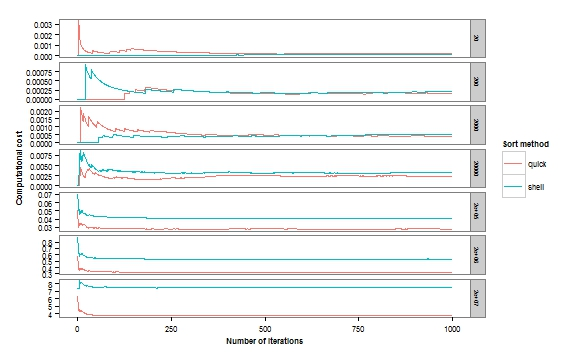
\includegraphics[scale=0.6]{Fig6.jpeg}
\caption{}
\end{centering}
\end{figure}
\end{itemize}
The above plot shows that for $n\leq20000$, estimates of time complexities for both quicksort and shellsort converge to similar values. In fact shellsort converges faster compared to quicksort for low $n$. But as $n$ increases this difference becomes wider and wider and shellsort takes considerably more time. We will see in part (e) that this behaviour agrees with the analytical results on run times for these algorithms. 

\item The worst case scenario for the time complexity of both quick sort and shell sort is $O(n^2)$. The best case scenario for quicksort and shellsort are $O(nlog(n))$ and $O(nlog^2(n))$ respectively. Plotting the estimates as a function of n and comparing this with the theoretical time complexities for both quicksort and shellsort. Here we plot the the ratio of our MC estimates with theoretical time complexities (for best case) vs. n for both the methods.
\begin{figure}[H]
\begin{centering}
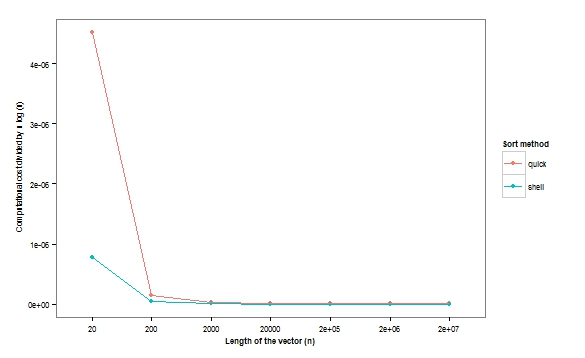
\includegraphics[scale=0.6]{Fig7.jpeg}
\caption{}
\end{centering}
\end{figure}

The above plot shows that for quicksort since this ratio converges to zero, $\dfrac{\overline{t_n}}{nlog(n)}=o(1)$. Clearly this implies we can choose any value as an upper bound i.e. $\dfrac{\overline{t_n}}{nlog(n)}=O(1)$. Similar reasoning for shellsort leads us to conclude that $\dfrac{\overline{t_n}}{nlog^2(n)}=O(1)$. Thus we can conclude that results from simulation agree with the analytical results.

\end{enumerate}

\section*{Answer 2}
Please see the file "aua257HW1.py" for Python code.

\section*{Answer 3}
\begin{enumerate}[label=(\alph*)]
\item Please see the file "aua257HW1.py" for Python code.
\item The value of the sum of squares is $5103133479.22$.

\end{enumerate}
\end{document}
